\documentclass[tikz,border=10pt]{standalone}
\usepackage{amsmath}
\usetikzlibrary{arrows.meta, positioning, calc, decorations.pathreplacing}
\definecolor{c1}{HTML}{000000}
\definecolor{c2}{HTML}{233D4D}
\definecolor{c3}{HTML}{FE7F2D}
\definecolor{c4}{HTML}{EAECF0}
\definecolor{axiscolor}{HTML}{333333}
\definecolor{labelcolor}{HTML}{5F6B75}
\begin{document}
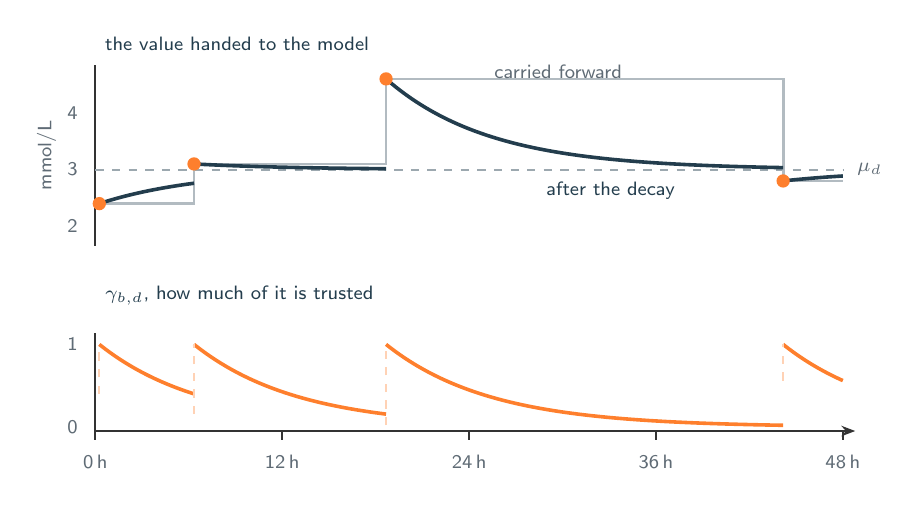
\begin{tikzpicture}[
    every node/.style={font=\sffamily},
    lab/.style={font=\sffamily\scriptsize, text=labelcolor},
    tag/.style={font=\sffamily\scriptsize, text=c2},
    hot/.style={font=\sffamily\scriptsize, text=c3!85!black},
]
\def\X#1{1.40 + #1*0.003300}
\def\Y#1{3.30 + (#1-2.0)*0.72}
\def\G#1{0.75 + #1*1.05}

% ================================================================ upper: the value
\node[tag, anchor=west] at (1.40, 5.62) {the value handed to the model};

\draw[axiscolor, line width=0.7pt] (1.40, 3.05) -- (1.40, 5.35);
\foreach \v in {2, 3, 4}{ \node[lab, anchor=east] at (1.30, {\Y{\v}}) {\v}; }
\node[lab, rotate=90] at (0.78, 4.20) {mmol/L};

% the channel mean
\draw[c2!45, line width=0.7pt, dashed] (1.40, {\Y{3.0}}) -- (10.90, {\Y{3.0}});
\node[lab, anchor=west] at (10.95, {\Y{3.0}}) {$\mu_d$};

% forward fill, for comparison
\draw[c2!35, line width=1.0pt]
    ({\X{15}}, {\Y{2.4}}) -- ({\X{380}}, {\Y{2.4}}) -- ({\X{380}}, {\Y{3.1}})
    -- ({\X{1120}}, {\Y{3.1}}) -- ({\X{1120}}, {\Y{4.6}})
    -- ({\X{2650}}, {\Y{4.6}}) -- ({\X{2650}}, {\Y{2.8}}) -- ({\X{2880}}, {\Y{2.8}});
\node[lab, anchor=west] at ({\X{1500}}, {\Y{4.72}}) {carried forward};

% the decayed value
\foreach \a/\b/\v in {15/380/2.4, 380/1120/3.1, 1120/2650/4.6, 2650/2880/2.8}{
    \draw[c2, line width=1.3pt]
        plot[domain=\a:\b, samples=80, smooth]
        ({\X{\x}}, {\Y{3.0 + (\v-3.0)*exp(-0.0025*(\x-\a))}});
}
\node[tag, anchor=west] at ({\X{1700}}, {\Y{2.62}}) {after the decay};

\foreach \m/\v in {15/2.4, 380/3.1, 1120/4.6, 2650/2.8}{
    \fill[c3] ({\X{\m}}, {\Y{\v}}) circle (2.4pt);
}

% ================================================================ lower: gamma
\node[tag, anchor=west] at (1.40, 2.42) {$\gamma_{b,d}$, how much of it is trusted};

\draw[axiscolor, line width=0.7pt] (1.40, 0.70) -- (1.40, 1.95);
\node[lab, anchor=east] at (1.30, {\G{0}}) {0};
\node[lab, anchor=east] at (1.30, {\G{1}}) {1};

\foreach \a/\b in {15/380, 380/1120, 1120/2650, 2650/2880}{
    \draw[c3, line width=1.3pt]
        plot[domain=\a:\b, samples=80, smooth]
        ({\X{\x}}, {\G{exp(-0.0025*(\x-\a))}});
    \draw[c3!35, line width=0.8pt, dashed]
        ({\X{\a}}, {\G{exp(-0.0025*(\b-\a))}}) -- ({\X{\a}}, {\G{1}});
}

% ================================================================ axis
\draw[axiscolor, line width=0.8pt, -{Stealth[length=5pt]}] (1.40, 0.70) -- (11.05, 0.70);
\foreach \h in {0, 12, 24, 36, 48}{
    \pgfmathsetmacro\m{\h*60}
    \draw[axiscolor, line width=0.7pt] ({\X{\m}}, 0.70) -- ({\X{\m}}, 0.58);
    \node[lab, anchor=north] at ({\X{\m}}, 0.52) {\h\,h};
}
\end{tikzpicture}
\end{document}
